\documentclass[11pt,a4paper]{article}
\usepackage[utf8]{inputenc}
\usepackage[T1]{fontenc}
\usepackage[english]{babel}
\usepackage[a4paper,margin=2.5cm]{geometry}
\usepackage{graphicx}
\usepackage{subcaption}
\usepackage{tikz}
\usepackage{hyperref}
\usepackage{enumitem}
\usepackage{parskip}
\usepackage{float}
\usepackage{placeins}

% Limit image height for very tall mobile mockups
\newcommand{\maxgraph}[2][]{% width optional, height fixed to 0.4\textheight
  \includegraphics[#1,height=0.4\textheight,keepaspectratio]
  {#2}%
}

\title{WeatherNow Calendar Integration\\\large Portfolio Assignment 02: UI/UX Design}
\author{
  \begin{tabular}{ll}
    Pascal Putz & \href{mailto:pascal.putz@study.thws.de}{pascal.putz@study.thws.de} (5123135)\\
    Gunn Kataria & \href{mailto:gunn.kataria@study.thws.de}{gunn.kataria@study.thws.de} (9125072)\\
    Katrina Alex & \href{mailto:katrina.alex@study.thws.de}{katrina.alex@study.thws.de} (9125071)\\
    Manuel Stöth & \href{mailto:manuel.stoeth@study.thws.de}{manuel.stoeth@study.thws.de} (5123045)\\
    Marvin Kraus & \href{mailto:marvin.kraus@study.thws.de}{marvin.kraus@study.thws.de} (5123143)
  \end{tabular}
}
\date{May 2025}

\begin{document}

\maketitle
\tableofcontents

\newpage

\section{Summary of Requirements}
Based on our Requirements Document, WeatherNow Calendar Integration is a React.js web application that combines real-time weather data (via OpenWeatherMap API) with the user’s Google Calendar (via Google Calendar API) to suggest context-aware activities. It must:

\begin{itemize}[noitemsep]
  \item Display current weather and a 5-day forecast for any city or geolocation.
  \item Integrate Google Calendar to detect free/busy slots for scheduling suggestions.
  \item Recommend personalized indoor or outdoor activities according to weather conditions and user availability.
  \item Provide a toggle between light and dark themes and a unit switch (°C/\textdegree F).
  \item Ensure responsive design across devices with accessible navigation to Home, Forecast, and Calendar views.
  \item Handle errors gracefully, including invalid input, permission denials, and API failures.
\end{itemize}

\section{User Interface Design}
This section presents mid-fidelity desktop and mobile mockups for the key screens: Home, Forecast, and Calendar. Each view is shown in light and dark variants, with mobile versions demonstrating responsive stacking and touch improvements.

\subsection{Home Screen}
\FloatBarrier
\begin{figure}[H]
  \centering
  \begin{subfigure}{0.48\linewidth}
    \includegraphics[width=\linewidth]{home_lightmode.jpeg}
    \caption{Desktop Light Mode}
  \end{subfigure}\hfill
  \begin{subfigure}{0.48\linewidth}
    \includegraphics[width=\linewidth]{home_darkmode.jpeg}
    \caption{Desktop Dark Mode}
  \end{subfigure}
  \caption{Home screen (desktop) with search, theme toggle, and summary of current weather and calendar suggestions.}
  \label{fig:home_desktop}
\end{figure}
\FloatBarrier

\subsubsection*{Mobile View}
\FloatBarrier
\begin{figure}[H]
  \centering
  \begin{subfigure}{0.48\linewidth}
    \maxgraph[width=\linewidth]{home_lightmode_mobile.jpg}
    \caption{Mobile Light Mode}
  \end{subfigure}\hfill
  \begin{subfigure}{0.48\linewidth}
    \maxgraph[width=\linewidth]{home_darkmode_mobile.jpg}
    \caption{Mobile Dark Mode}
  \end{subfigure}
  \caption{Mobile Home screen with vertical stacking, larger touch targets, and simplified header controls.}
  \label{fig:home_mobile}
\end{figure}
\FloatBarrier

\subsection{Forecast Screen}
\FloatBarrier
\begin{figure}[H]
  \centering
  \begin{subfigure}{0.48\linewidth}
    \includegraphics[width=\linewidth]{forecast_lightmode.jpeg}
    \caption{Desktop Light Mode}
  \end{subfigure}\hfill
  \begin{subfigure}{0.48\linewidth}
    \includegraphics[width=\linewidth]{forecast_darkmode.jpeg}
    \caption{Desktop Dark Mode}
  \end{subfigure}
  \caption{5-day weather forecast (desktop) with interval cards, icons, and summary metric.}
  \label{fig:forecast_desktop}
\end{figure}
\FloatBarrier

\subsubsection*{Mobile View}
\FloatBarrier
\begin{figure}[H]
  \centering
  \begin{subfigure}{0.48\linewidth}
    \maxgraph[width=\linewidth]{forecast_lightmode_mobile.jpg}
    \caption{Mobile Light Mode}
  \end{subfigure}\hfill
  \begin{subfigure}{0.48\linewidth}
    \maxgraph[width=\linewidth]{forecast_darkmode_mobile.jpg}
    \caption{Mobile Dark Mode}
  \end{subfigure}
  \caption{Mobile forecast with full-width stacked cards for each interval, optimized for scrolling.}
  \label{fig:forecast_mobile}
\end{figure}
\FloatBarrier

\subsection{Calendar \& Planner Screen}
\FloatBarrier
\begin{figure}[H]
  \centering
  \begin{subfigure}{0.48\linewidth}
    \includegraphics[width=\linewidth]{calendar_lightmode.jpeg}
    \caption{Desktop Light Mode}
  \end{subfigure}\hfill
  \begin{subfigure}{0.48\linewidth}
    \includegraphics[width=\linewidth]{calendar_darkmode.jpeg}
    \caption{Desktop Dark Mode}
  \end{subfigure}
  \caption{Calendar view (desktop) showing selectable dates, event slots, weather overlay, and suggested activities.}
  \label{fig:calendar_desktop}
\end{figure}
\FloatBarrier

\subsubsection*{Mobile View}
\FloatBarrier
\begin{figure}[H]
  \centering
  \begin{subfigure}{0.48\linewidth}
    \maxgraph[width=\linewidth]{calendar_lightmode_mobile.jpg}
    \caption{Mobile Light Mode}
  \end{subfigure}\hfill
  \begin{subfigure}{0.48\linewidth}
    \maxgraph[width=\linewidth]{calendar_darkmode_mobile.jpg}
    \caption{Mobile Dark Mode}
  \end{subfigure}
  \caption{Mobile calendar with bottom tab navigation, single-column layout, and compact event display.}
  \label{fig:calendar_mobile}
\end{figure}
\FloatBarrier

\section{Navigation Flow}
\FloatBarrier
\begin{figure}[H]
  \centering
  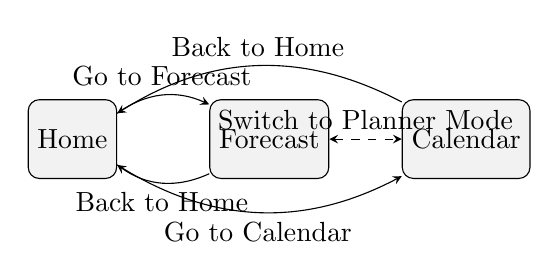
\begin{tikzpicture}[node distance=2.5cm, auto, >=stealth]
    \tikzstyle{screen}=[rectangle,draw,rounded corners,minimum height=1cm,fill=gray!10]
    \node[screen] (home){Home};
    \node[screen,right of=home] (forecast){Forecast};
    \node[screen,right of=forecast] (calendar){Calendar};
    \path[->](home)edge[bend left]node[above]{Go to Forecast}(forecast);
    \path[->](forecast)edge[bend left]node[below]{Back to Home}(home);
    \path[->](home)edge[bend right]node[below]{Go to Calendar}(calendar);
    \path[->](calendar)edge[bend right]node[above]{Back to Home}(home);
    \path[<->,dashed](forecast)edge node[above]{Switch to Planner Mode}(calendar);
  \end{tikzpicture}
  \caption{User navigation illustrating consistent, intuitive flow between screens.}
  \label{fig:flow}
\end{figure}
\FloatBarrier

\section{Design Decisions and Rationale}
This section explains the reasoning behind key UI conventions and patterns chosen to meet user needs and requirements.

\subsection{Hierarchy and Layout}
We use a clean header with persistent tabs to ensure users can quickly switch between Home, Forecast, and Calendar (addressing clarity and discoverability). Information is grouped within card components for weather summaries, forecast intervals, and calendar events, creating a clear visual hierarchy and supporting glanceable insights.

\subsection{Theming and Customization}
A light/dark mode toggle respects individual preferences and environmental lighting conditions (enhancing readability and reducing eye strain). The unit switch (°C/\textdegree F) supports regional user expectations, improving usability across different markets.

\subsection{Responsive Behavior}
Layouts adapt from a two-column desktop view to a single-column mobile view at breakpoints of 768px and 480px. On mobile, cards are full-width with increased touch target sizes (minimum 44×44px), and navigation shifts to a bottom tab bar for ergonomic access.

\subsection{Error Handling and Accessibility}
Inline alerts and toast notifications provide immediate feedback for invalid city inputs or API issues, maintaining user trust. All interactive elements include ARIA labels and logical tabindex ordering, ensuring operability via assistive technologies and keyboard navigation. Color contrast ratios exceed WCAG 2.1 AA thresholds for readability.

\section{Evaluation Against Criteria}
\subsection{Clarity and Completeness of the Design}
Each screen is presented with labeled visuals and accompanied by descriptive captions and explanatory text. The Home, Forecast, and Calendar views are understandable in isolation and in context, illustrating all core functionalities.

\subsection{Consistency and Structure of Navigation}
The navigation diagram (Fig.~\ref{fig:flow}) shows a consistent, intuitive flow. Primary tabs remain in a fixed header on desktop and a bottom bar on mobile, reinforcing user goals and minimizing cognitive load.

\subsection{Visual and Interaction Design Quality}
Cards, whitespace, and typography have been used to emphasize content hierarchy. Established UI patterns (tabs, cards, toggles) ensure familiarity. Interaction elements are clearly indicated with bold buttons and icons, providing affordances for user actions.

\subsection{Connection to Requirements and User Needs}
Design rationale sections map directly to user stories and requirements: theme toggles satisfy preference needs (US6), calendar integration addresses scheduling stories, and errors are handled per US7. Recommendations panels link weather data to actionable items, reflecting user-centric functionality.

\section*{Acknowledgement of AI Technologies}
This document was drafted and refined using GPT-4o based on outlines and reviewed by all authors.

\end{document}
